\begin{figure}
\centering
\def\layersep{3cm}
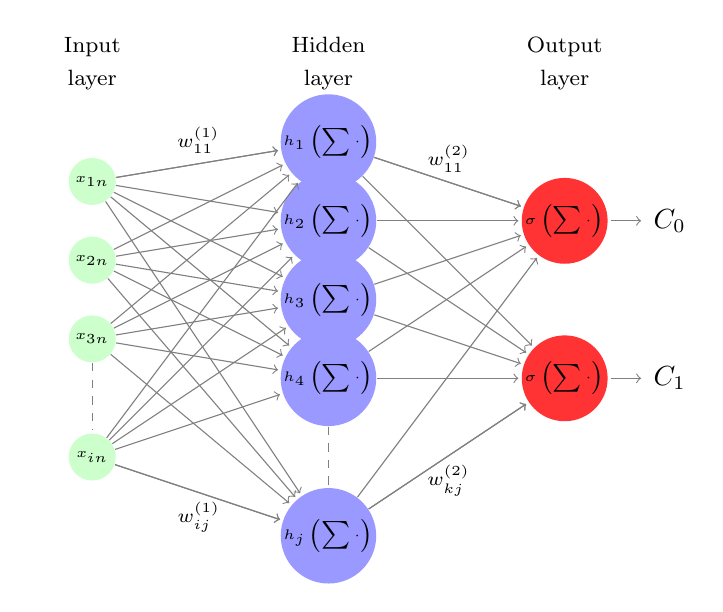
\begin{tikzpicture}[shorten >=1pt,draw=black!50, node distance=\layersep]
    \tikzstyle{every pin edge}=[<-,shorten <=1pt]
    \tikzstyle{neuron}=[circle,fill=black!25,minimum size=17pt,inner sep=0pt]
    \tikzstyle{input neuron}=[neuron, fill=green!20];
    \tikzstyle{output neuron}=[neuron, fill=red!80];
    \tikzstyle{hidden neuron}=[neuron, fill=blue!40];
    \tikzstyle{annot} = [text width=4em, text centered]

    % Draw the input layer nodes
    \foreach \name / \y in {1,...,3}
    % This is the same as writing \foreach \name / \y in {1/1,2/2,3/3,4/4}
        \node[input neuron] (I-\name) at (0,-\y) {\tiny $x_{ \y n }$};
        
   \node[input neuron] (I-4) at (0,-4.5) {\tiny $x_{in}$};
   \draw[dashed,draw=black!50] (I-3) -- (I-4);

    % Draw the hidden layer nodes
    \foreach \name / \y in {1,...,4}
        \path[yshift=0.5cm]
            node[hidden neuron] (H-\name) at (\layersep,-\y cm) {\tiny $h_{ \y }\left(\sum \cdot \right)$};
            
    \node[hidden neuron] (H-5) at (\layersep,-5.5 cm) {\tiny $h_{j}\left(\sum \cdot \right)$};
    \draw[dashed,draw=black!50] (H-4) -- (H-5);

    % Draw the output layer node
    	\node[output neuron,pin={[pin edge={->}]right:$C_{0}$}, right of=H-2] (O-1) {\tiny $\sigma\left(\sum \cdot \right)$};
    	\node[output neuron,pin={[pin edge={->}]right:$C_{1}$}, right of=H-4] (O-2) {\tiny $\sigma\left(\sum \cdot \right)$};

    % Connect every node in the input layer with every node in the
    % hidden layer.
    \foreach \source in {1,...,4}
        \foreach \dest in {1,...,5}
        		\draw[shorten >=1pt,->,draw=black!50] (I-\source)  -- (H-\dest);
            %\path (I-\source) edge (H-\dest);
    
    % Draw the annotation for the weight for the first and last connections       
    \draw[shorten >=1pt,->,draw=black!50] (I-1) -- (H-1) node [midway, above] (w111) {\scriptsize $w_{11}^{(1)}$};
    \draw[shorten >=1pt,->,draw=black!50] (I-4) -- (H-5) node [midway, below] (w145) {\scriptsize $w_{ij}^{(1)}$};

    % Connect every node in the hidden layer with the output layer
    \foreach \source in {1,...,5}
    		\foreach \dest in {1,...,2}
        		\draw[shorten >=1pt,->,draw=black!50] (H-\source)  -- (O-\dest);
        %\path (H-\source) edge (O);
        
    % Draw the annotation for the weight for the first and last connections       
    \draw[shorten >=1pt,->,draw=black!50] (H-1) -- (O-1) node [midway, above] (w211) {\scriptsize $w_{11}^{(2)}$};
    \draw[shorten >=1pt,->,draw=black!50] (H-5) -- (O-2) node [midway, below] (w251) {\scriptsize $w_{kj}^{(2)}$};

    % Annotate the layers
    \node[annot,above of=H-1, node distance=1cm] (hl) {\footnotesize Hidden layer};
    \node[annot,left of=hl] {\footnotesize Input layer};
    \node[annot,right of=hl] {\footnotesize Output layer};
\end{tikzpicture}
\caption{Representation of a neural network of the multilayer perceptron family.}
\label{fig:mlp}
\end{figure}
